\documentclass[10pt,xcolor={dvipsnames}]{beamer}
\usetheme[
%%% option passed to the outer theme
%    progressstyle=fixedCircCnt,   % fixedCircCnt, movingCircCnt (moving is deault)
  ]{Feather}
  
% If you want to change the colors of the various elements in the theme, edit and uncomment the following lines


\definecolor{NavyBlue}{rgb}{0.0, 0.47, 0.75} %azul
%\definecolor{NavyBlue}{rgb}{1.0, 0.35, 0.21} %naranja
%\definecolor{NavyBlue}{rgb}{0.63, 0.36, 0.94} %morado
%\definecolor{NavyBlue}{rgb}{0.8, 0.6, 0.8} %rosado
  
% Change the bar colors:
\setbeamercolor{Feather}{fg=NavyBlue!20,bg=NavyBlue}

% Change the color of the structural elements:
\setbeamercolor{structure}{fg=NavyBlue}

% Change the frame title text color:
\setbeamercolor{frametitle}{fg=black!5}

% Change the normal text colors:
\setbeamercolor{normal text}{fg=black!75,bg=gray!5}

%% Change the block title colors
\setbeamercolor{block title}{use=Feather,bg=Feather.fg, fg=black!90} 


% Change the logo in the upper right circle:
%\renewcommand{\logofile}{example-grid-100x100pt} 
%% This is an image that comes with the LaTeX installation
% Adjust scale of the logo w.r.t. the circle; default is 0.875
% \renewcommand{\logoscale}{0.55}

% Change the background image on the title and final page.
% It stretches to fill the entire frame!
% \renewcommand{\backgroundfile}{example-grid-100x100pt}

%-------------------------------------------------------
% INCLUDE PACKAGES
%-------------------------------------------------------

\usepackage[utf8]{inputenc}
\usepackage[english]{babel}
\usepackage[T1]{fontenc}
% \usepackage{helvet}

%% Load different font packages to use different fonts
%% e.g. using Linux Libertine, Linux Biolinum and Inconsolata
% \usepackage{libertine}
% \usepackage{zi4}

%% e.g. using Venturis ADF Serif and Sans
% \usepackage{venturis}

%-------------------------------------------------------
% DEFFINING AND REDEFINING COMMANDS
%-------------------------------------------------------

% colored hyperlinks
\newcommand{\chref}[2]{
  \href{#1}{{\usebeamercolor[bg]{Feather}#2}}
}

%-------------------------------------------------------
% INFORMATION IN THE TITLE PAGE
%-------------------------------------------------------

\title[Fund Computación] % [] is optional - is placed on the bottom of the sidebar on every slide
{ % is placed on the title page
      \Large{\textbf{Fundamentación en computación}}
}

\subtitle[Clase 3]
{
      \textbf{Una herramienta científica inevitable}
}

\author[Julián Calle]
{      Julián Calle \\
      {\ttfamily julian.callem@udea.edu.co}\\[1em]
      Clase 3
}

\institute[UdeA]
{%
\begin{columns}
\begin{column}{3cm}

\includegraphics[scale=0.045]{Feathergraphics/2-2} 
\end{column}
\begin{column}{6cm} 
Instituto de física\\
Facultad de ciencias exactas y naturales \\
Universidad de Antioquia
\end{column} \end{columns}
}

\date{\today}

%-------------------------------------------------------
% THE BODY OF THE PRESENTATION
%-------------------------------------------------------

\begin{document}

%-------------------------------------------------------
% THE TITLEPAGE
%-------------------------------------------------------

{\1
\begin{frame}[plain,noframenumbering]
  \titlepage
\end{frame}}


\begin{frame}{Content}{}
\tableofcontents
\end{frame}

\begin{frame}
\begin{center}
\Large{\textcolor{blue}{¿Cómo una computadores puede hacer tantas cosas?}} \pause

\includegraphics[scale=0.3]{Figures/1Duda}
\end{center}
\end{frame}

\begin{frame}{Introducción}
\begin{center}
\only<1>{\Large{Trabajar} \\ 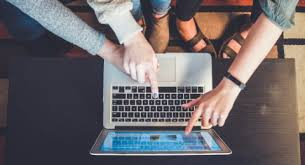
\includegraphics[scale=1.0]{Figures/1Trabajar}}
\only<2>{\Large{Jugar} \\ 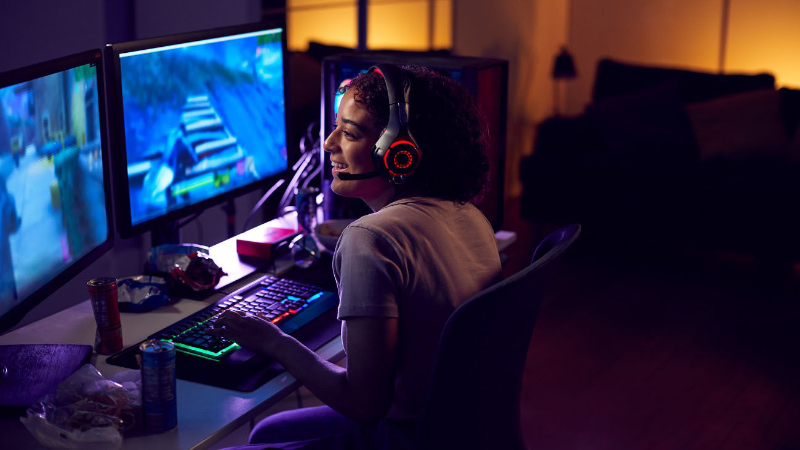
\includegraphics[scale=0.4]{Figures/1Jugar}}
\only<3>{\Large{Programar} \\ 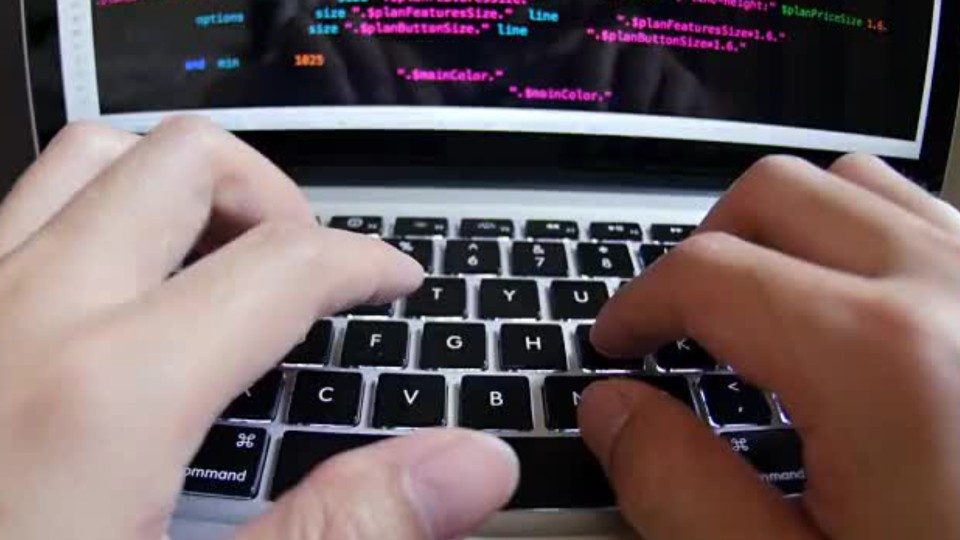
\includegraphics[scale=0.3]{Figures/1Programar}}
\only<4>{\Large{ETC.} \\ 
\includegraphics[scale=0.25]{Figures/1etc}}
\end{center}
\end{frame}

\begin{frame}{Introducción}
\begin{center}
\only<1>{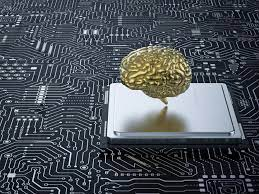
\includegraphics[scale=1.0]{Figures/1CPU2}}
\only<2>{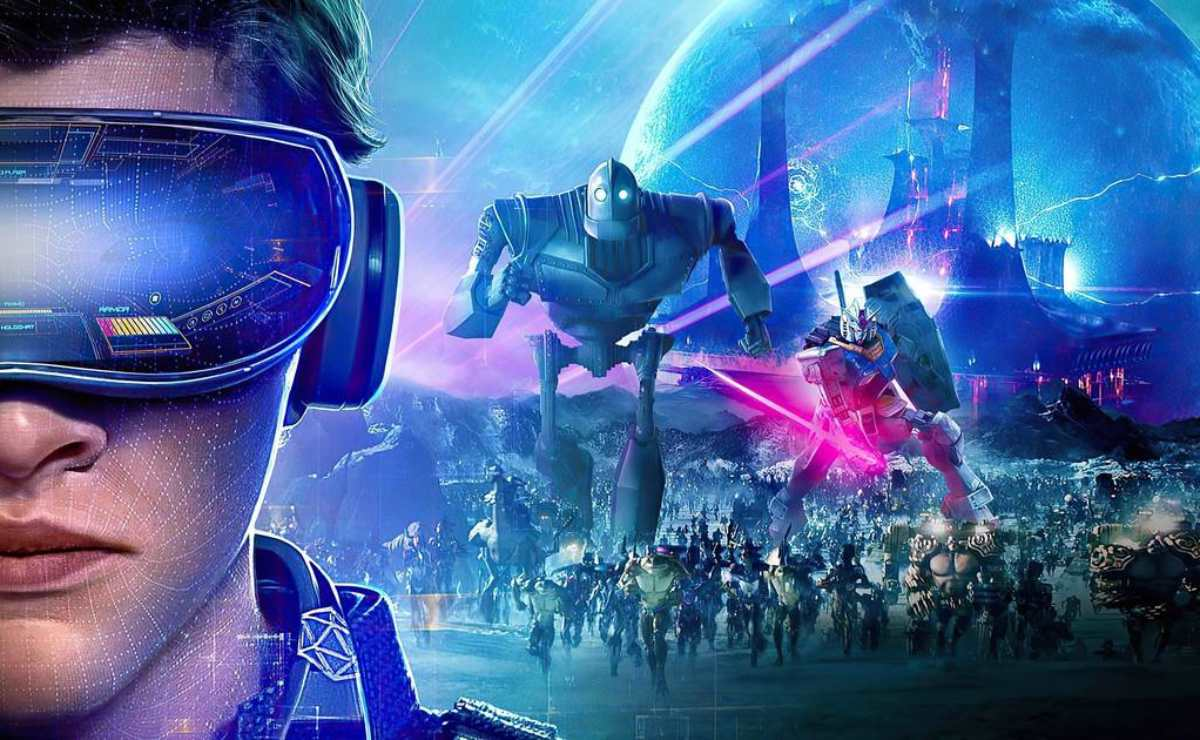
\includegraphics[scale=1.0]{Figures/1virtual}}
\only<3>{
\includegraphics[scale=0.3]{Figures/1PC}}
\only<4>{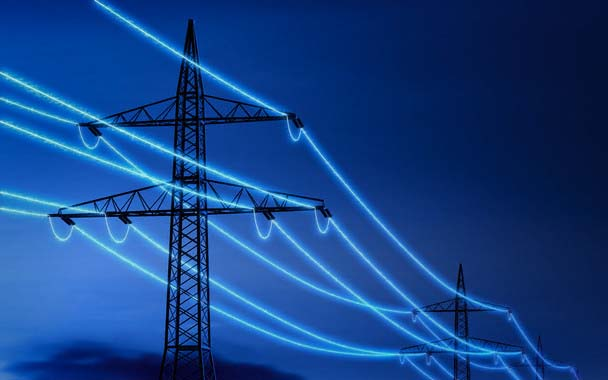
\includegraphics[scale=0.5]{Figures/1Electricidad}}
\only<5>{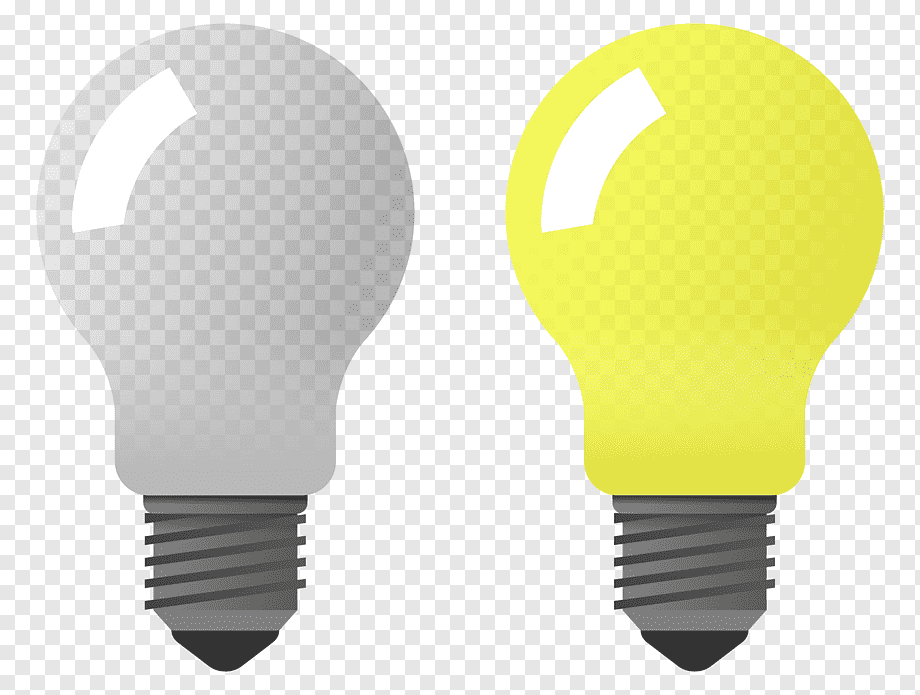
\includegraphics[scale=0.3]{Figures/1Bombilla}}
\only<6>{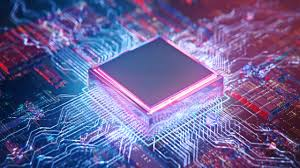
\includegraphics[scale=1.0]{Figures/1CPU}}
\end{center}
\end{frame}



\section{Sistemas de conteo}

\begin{frame}
\begin{center}
\Huge{\textcolor{blue}{Sistemas de conteo}} \\ \pause
\Large{\textcolor{red}{¿Cómo se cuenta?}}
\end{center}
\end{frame}


\begin{frame}
\begin{center}
\Huge{\textcolor{blue}{Sistema decimal}}
\end{center}
\end{frame}

\begin{frame}{Sistema decimal}
\begin{center}
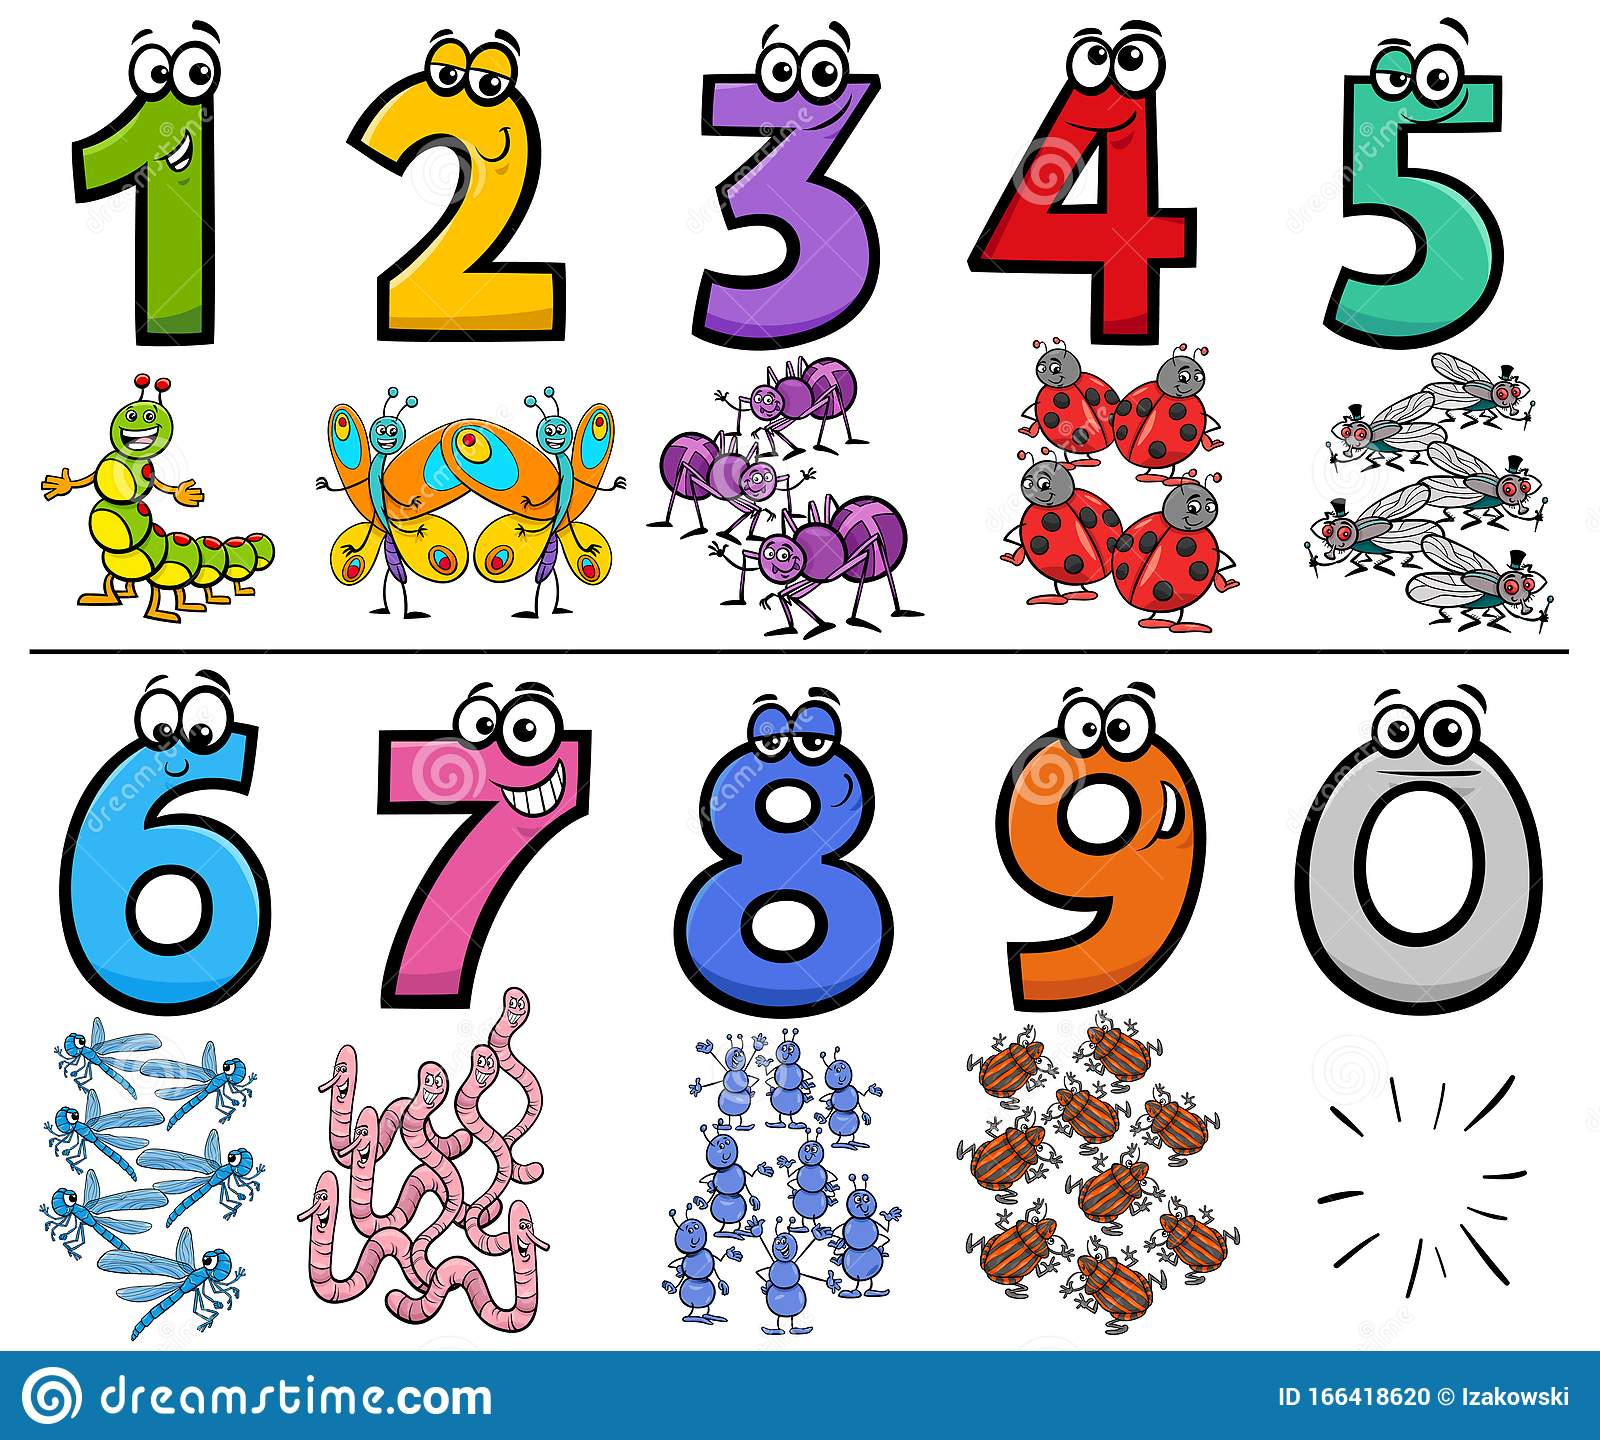
\includegraphics[scale=0.6]{Figures/2numeros}
\end{center}
\end{frame}

\begin{frame}{Sistema decimal}
\begin{center}
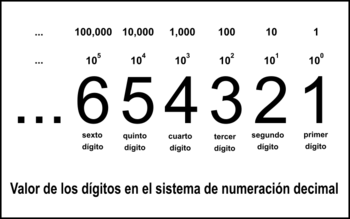
\includegraphics[scale=0.8]{Figures/2decimal} \\ \pause
\url{https://www.mathematik.uni-marburg.de/~thormae/lectures/ti1/code/abacus/soroban.html}
\end{center}
\end{frame}

\begin{frame}{Sistema hexadecimal}
\begin{center}
\Large{¿Qué pasaría si en lugar de 10 dedos tuvieramos 16?} \\ \pause
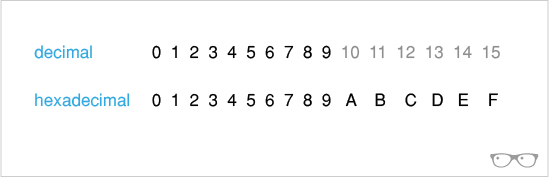
\includegraphics[scale=0.55]{Figures/2hexadecimales}
\end{center}
\end{frame}

\begin{frame}
\begin{center}
\Huge{\textcolor{blue}{Sistema binario}} \\ \vspace{0.5cm} \pause
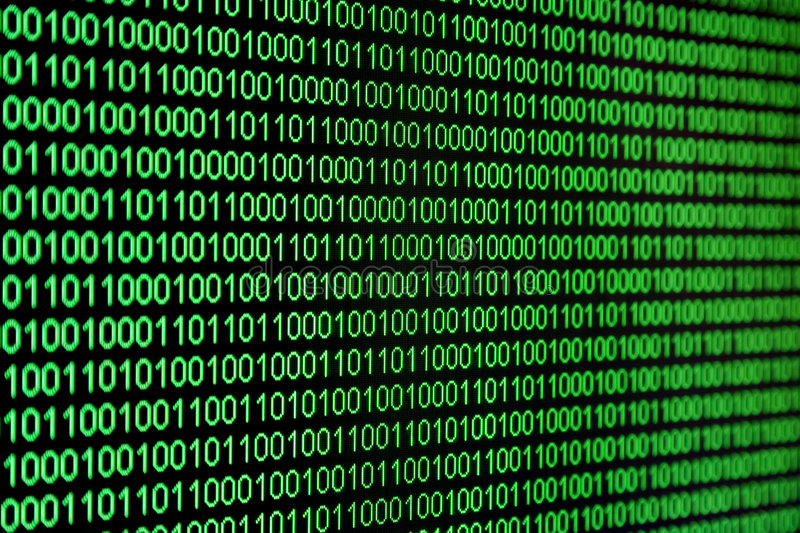
\includegraphics[scale=1.0]{Figures/2binario}
\end{center}
\end{frame}

\begin{frame}{Sistema binario}
\begin{center}
\only<1>{
\includegraphics[scale=0.7]{Figures/binario2}}
\only<2>{
\includegraphics[scale=0.6]{Figures/binario}}
\only<3->{\Large{Continuamos con más binarios la siguiente clase}}
\only<3->{
\includegraphics[scale=0.3]{Figures/Homero}}
\end{center}
\end{frame}

\begin{frame}{Equivalencias}
\begin{center}
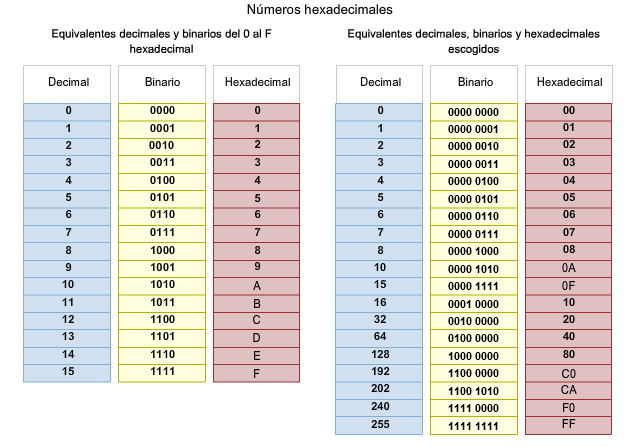
\includegraphics[scale=0.45]{Figures/2conteo}
\end{center}
\end{frame}

\section{Álgebra Booleana}

\begin{frame}
\begin{center}
\Huge{\textcolor{blue}{Álgebra Booleana}} \\ 
\only<2>{\vspace{0.5cm} 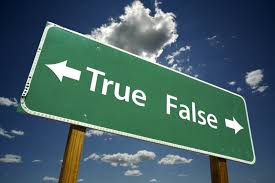
\includegraphics[scale=0.7]{Figures/3booleana} \\ \tiny{\url{https://bookdown.org/alberto_brunete/intro_automatica/algebraboole.html}}}
\end{center}
\end{frame}

\begin{frame}{Álgebra Booleana}
\begin{center}
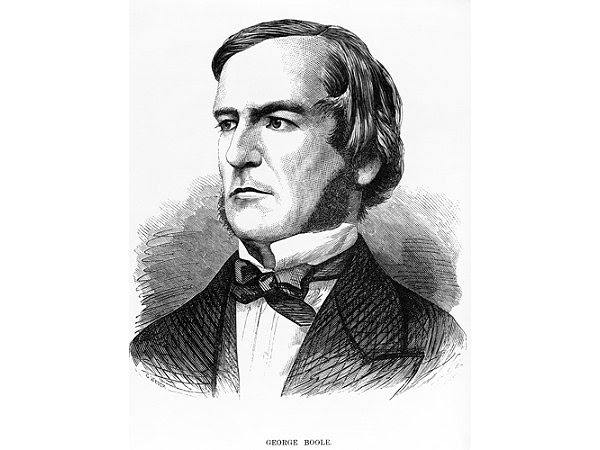
\includegraphics[scale=0.35]{Figures/3George-Boole} \\
George Boole (1815-1864)
\end{center}
\end{frame}


\begin{frame}{Álgebra Booleana}
\begin{center}
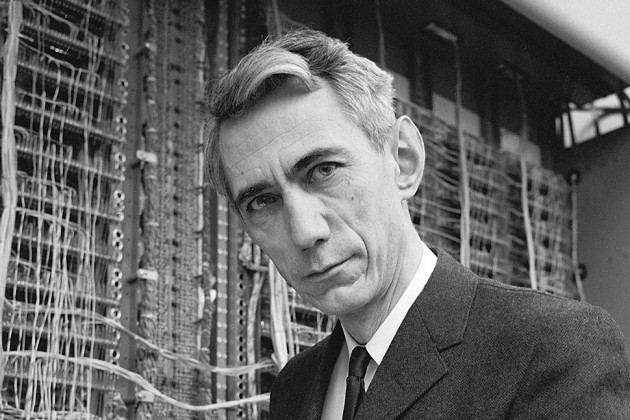
\includegraphics[scale=0.4]{Figures/3Shannon} \\
Claude Shannon (1916-2021)
\end{center}
\end{frame}


\begin{frame}{Álgebra Booleana}
\begin{center}
El álgebra de Boole o Booleana está formada por lo siguiente: \\ \pause
\only<1-2>{\Large{\textcolor{blue}{Dos variables}}\\}
\only<2>{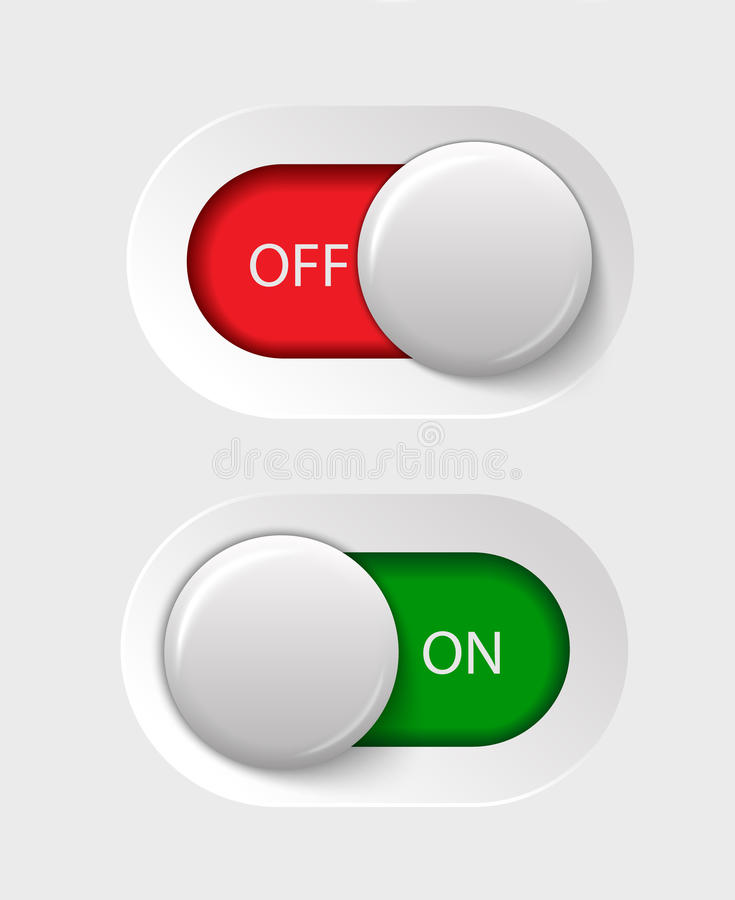
\includegraphics[scale=0.3]{Figures/3Binar1}
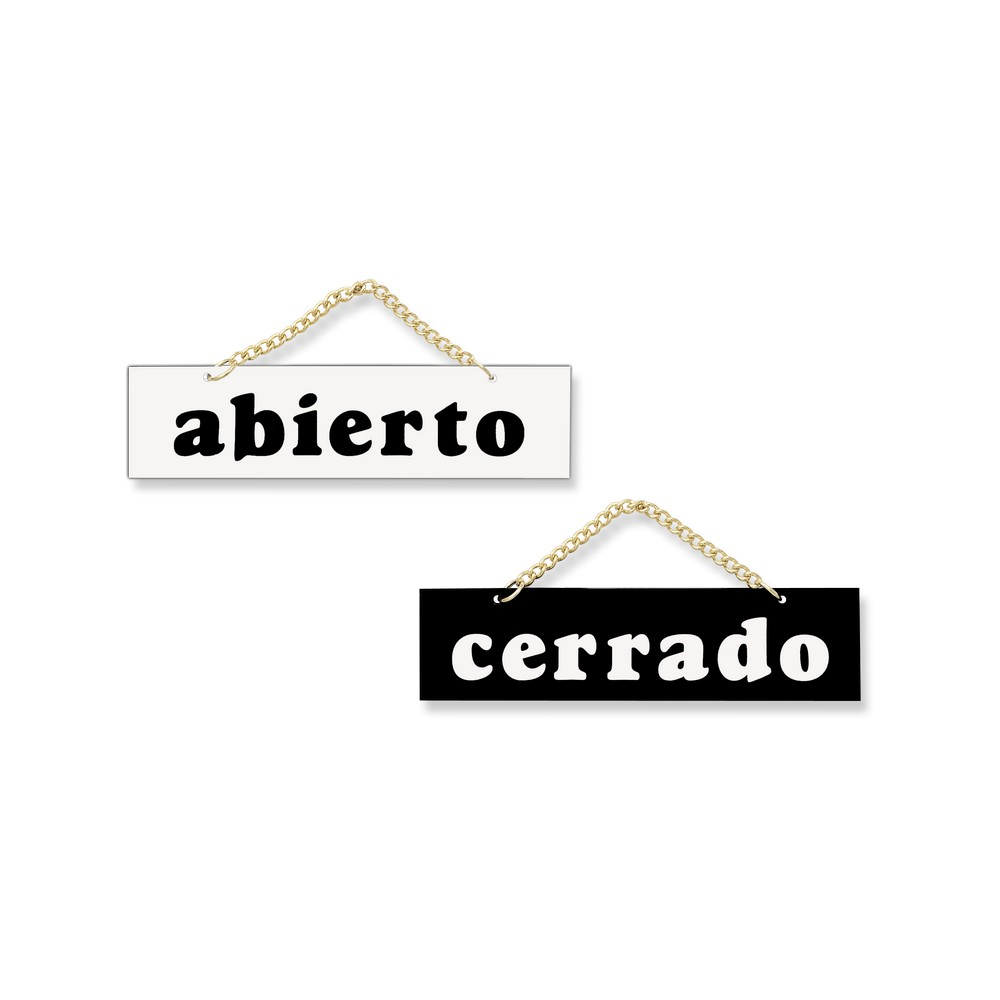
\includegraphics[scale=0.08]{Figures/3Binar}
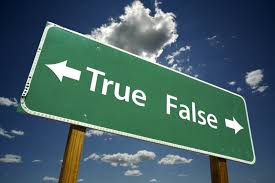
\includegraphics[scale=0.3]{Figures/3booleana}
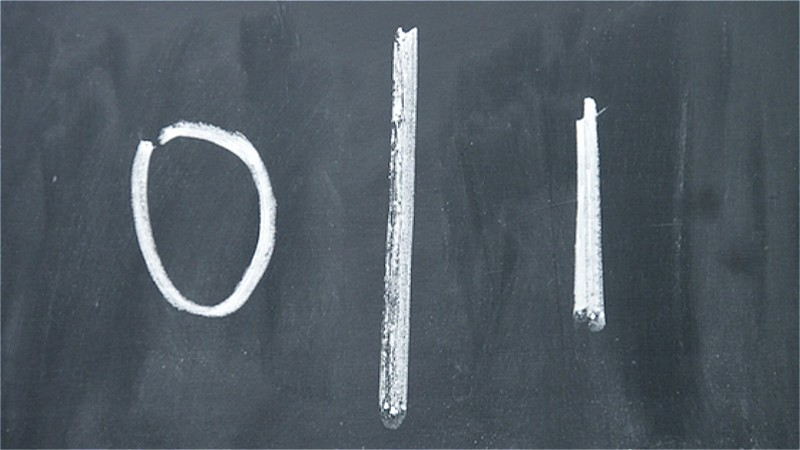
\includegraphics[scale=0.2]{Figures/3Bolean3}}
\only<3->{\Large{\textcolor{blue}{Tres operaciones \\}}}
\only<4-5>{\large{\textcolor{red}{Suma o OR \\}}}
\only<5>{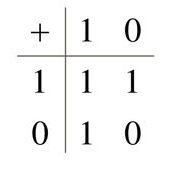
\includegraphics[scale=0.8]{Figures/3Suma}}
\only<6-7>{\large{\textcolor{red}{Multiplicación o AND \\}}}
\only<7>{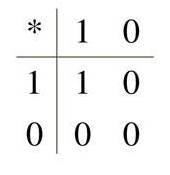
\includegraphics[scale=0.8]{Figures/3mult}}
\only<8-9>{\large{\textcolor{red}{Complemento o NOT \\}}}
\only<9>{
\begin{eqnarray}
	\overline{1} &= 0 \nonumber \\
	\overline{0} &= 1 \nonumber
\end{eqnarray}
}
\end{center}
\end{frame}

{\1
\begin{frame}[plain,noframenumbering]
  \finalpage{\Huge{Pausa}}
\end{frame}}


\begin{frame}
\begin{center}
\only<1>{\Huge{\textcolor{red}{¿En qué escala piensa tu cerebro?}}}
\only<2-6>{\Huge{\textcolor{blue}{¿Qué número hay entre 1 y 9?}}}
\only<3>{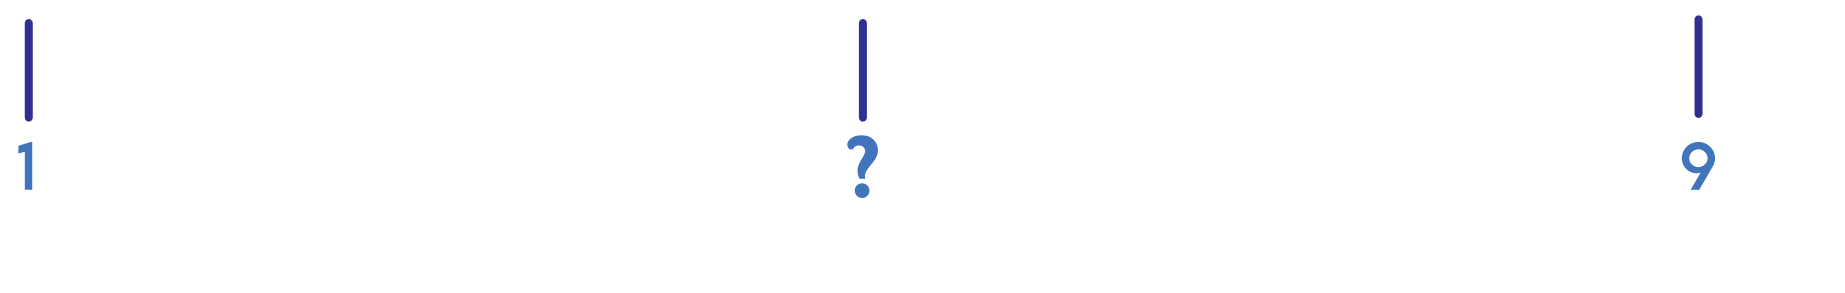
\includegraphics[scale=0.25]{Figures/LescalaPregunta}}
\only<4>{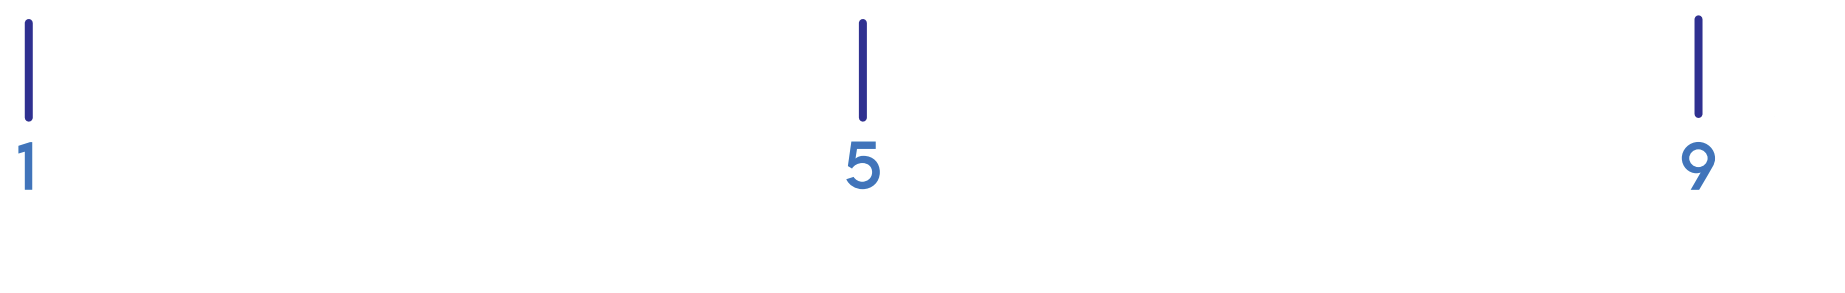
\includegraphics[scale=0.25]{Figures/Lescala5}}
\only<4>{\Large{$\approx 100\%$}}
\only<5>{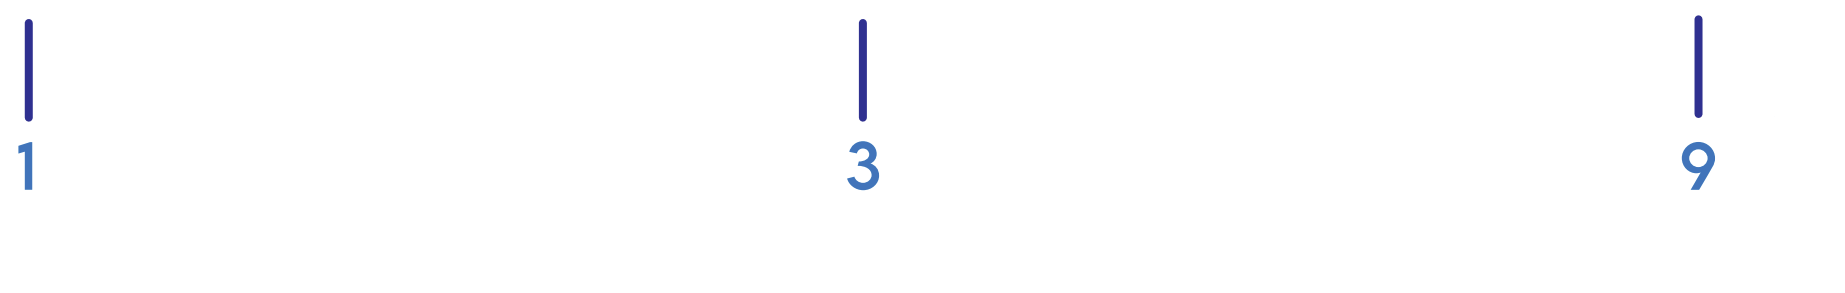
\includegraphics[scale=0.25]{Figures/Lescala3}}
\only<5>{\Large{¿Es posible?}}
\only<6>{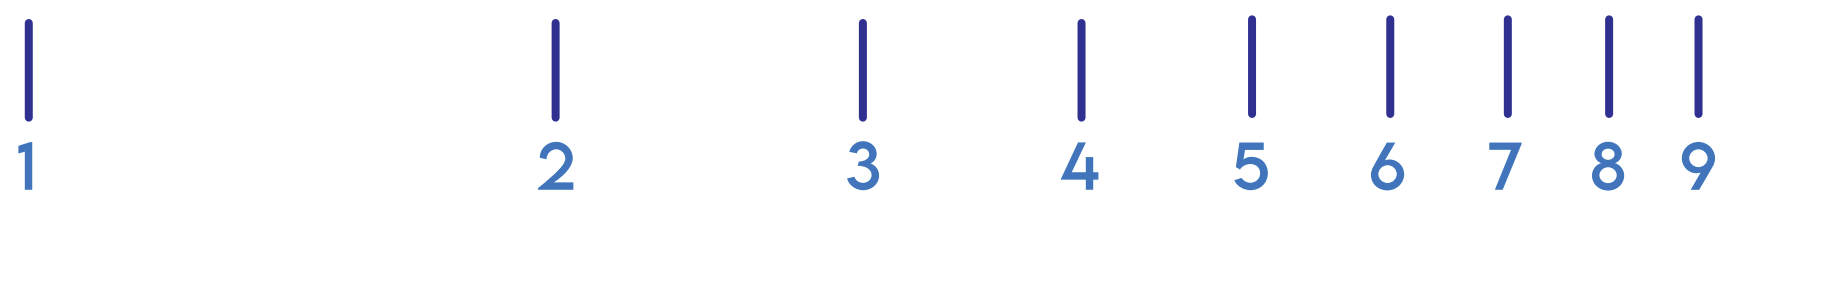
\includegraphics[scale=0.25]{Figures/Lescala9}}
\only<7>{Development of Numerical Estimation in Young Children \\
Robert S. Siegler and Julie L. Booth \\
Department of Psychology \\
Carnegie Mellon University.}
\only<7>{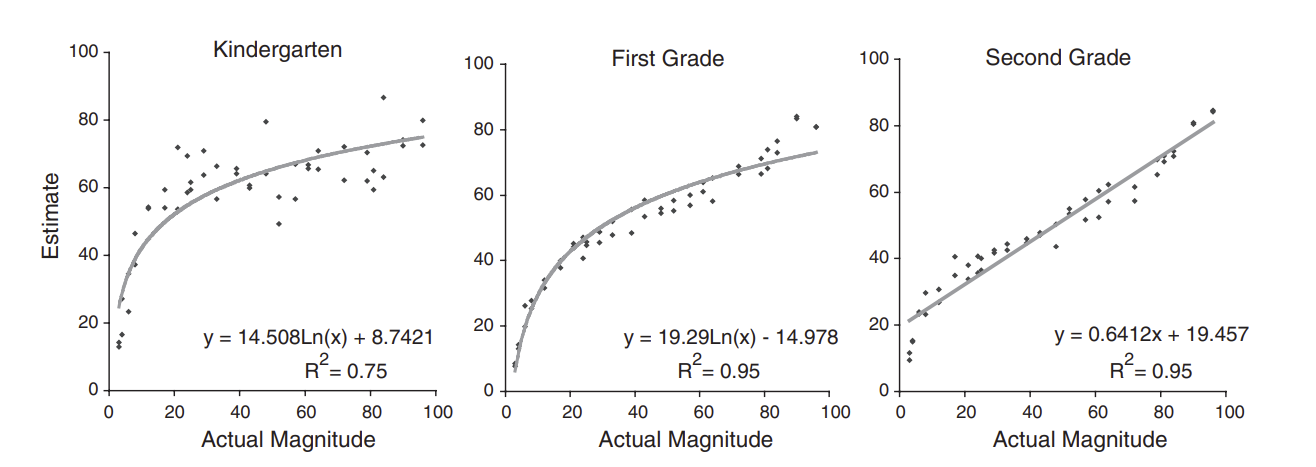
\includegraphics[scale=0.33]{Figures/estudio}}
\only<8>{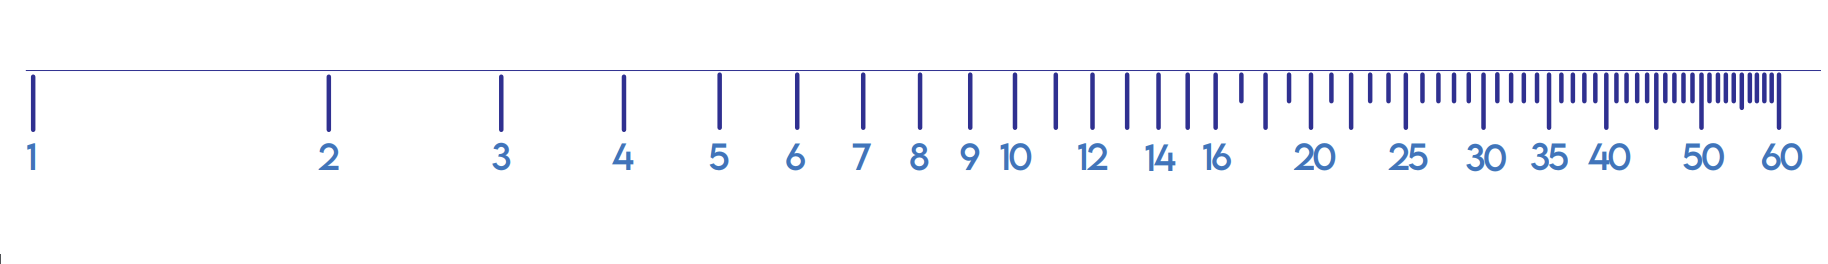
\includegraphics[scale=0.23]{Figures/Lescala}}
\only<8>{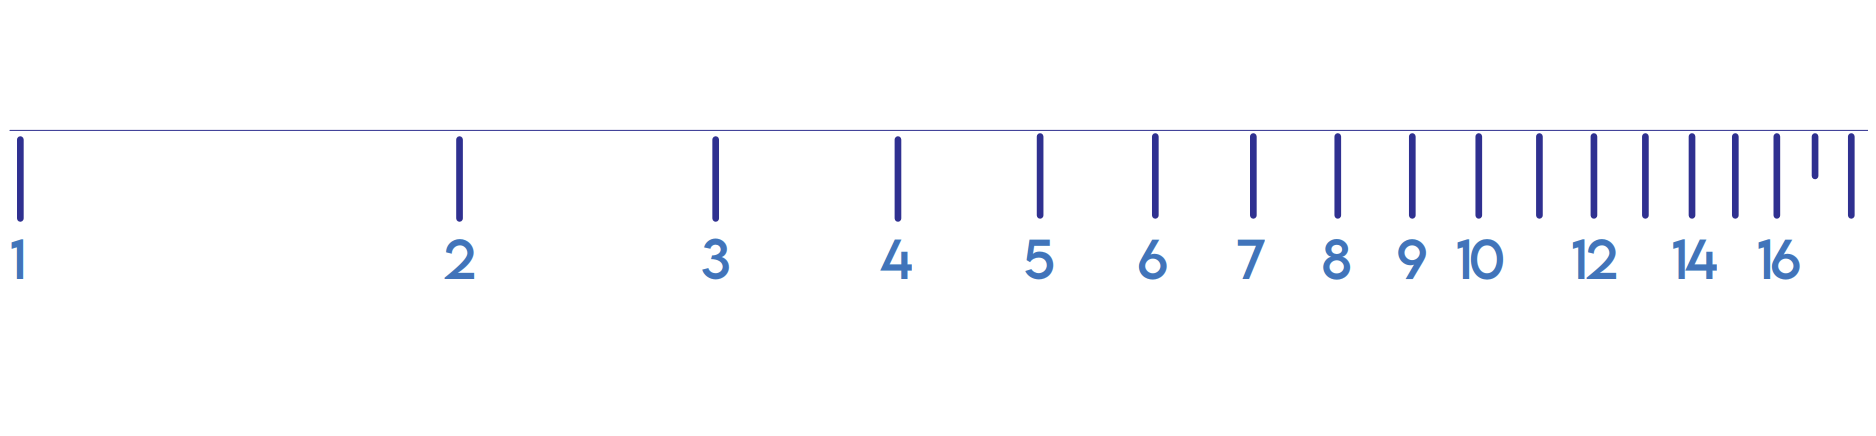
\includegraphics[scale=0.23]{Figures/Lescala18}}
\only<8>{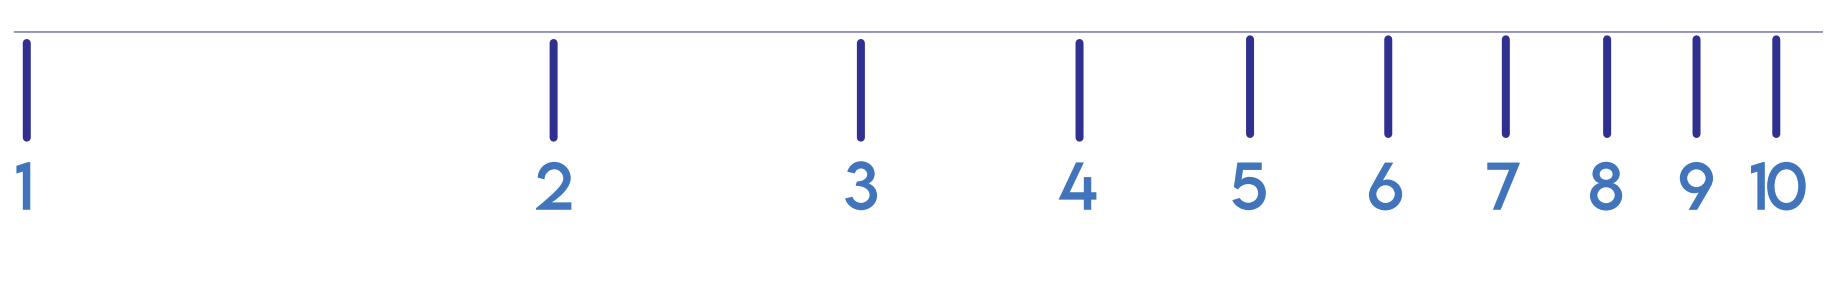
\includegraphics[scale=0.23]{Figures/Lescala10}}
\only<9-10>{\Large{¿Cómo se ve 10000 y  100000 años luz en una recta?}}
\only<10>{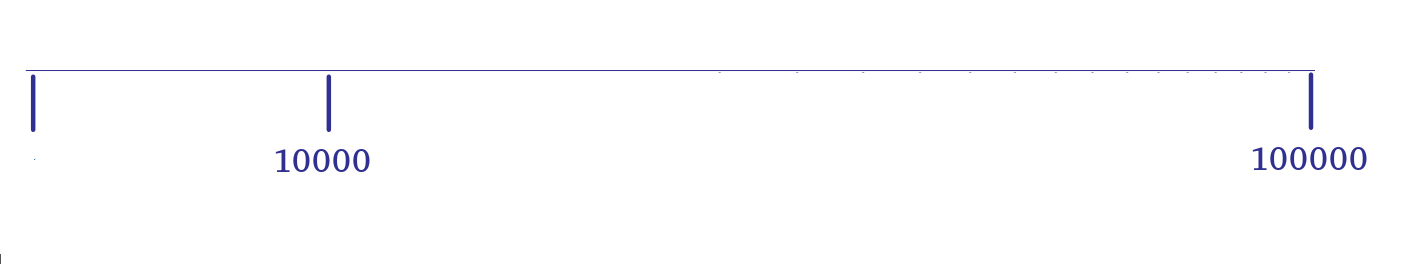
\includegraphics[scale=0.3]{Figures/LescalaDistancia}}
\end{center}
\end{frame}

{\1
\begin{frame}[plain,noframenumbering]
  \finalpage{\Huge{Retornamos}}
\end{frame}}


\section{Procesadores}

\begin{frame}
\begin{center}
\Huge{\textcolor{blue}{Procesador}}
\end{center}
\end{frame}

\begin{frame}{Procesador}
\begin{center}
\Huge{¿Cómo se fabrica un procesador?} \\ \pause
\tiny{\url{https://youtu.be/mrB3jAfpmEQ}}
\end{center}
\end{frame}

\begin{frame}{Procesador}
\begin{center}
\only<2>{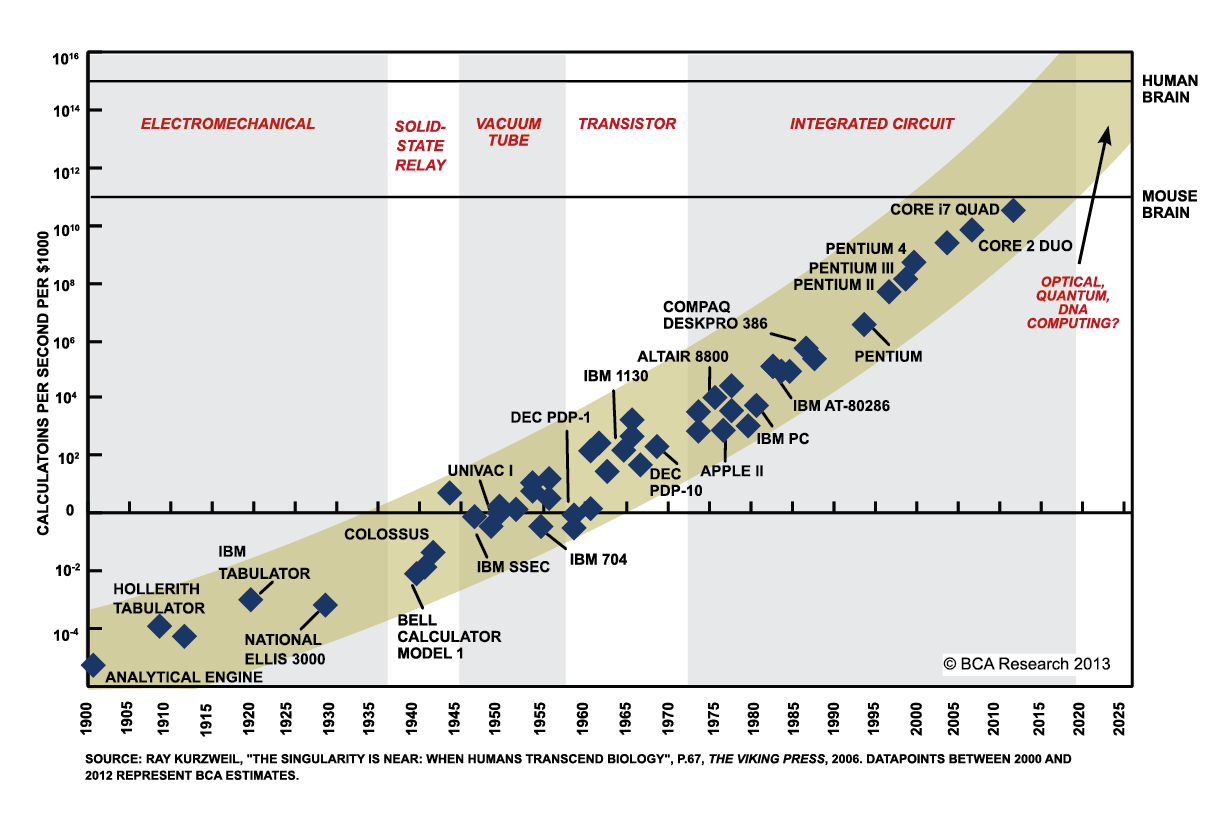
\includegraphics[scale=0.25]{Figures/MooresLaw2}}
\only<3>{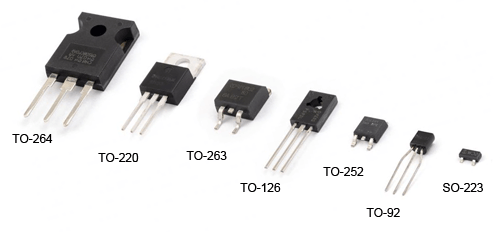
\includegraphics[scale=0.5]{Figures/transistorArd}}
\only<4>{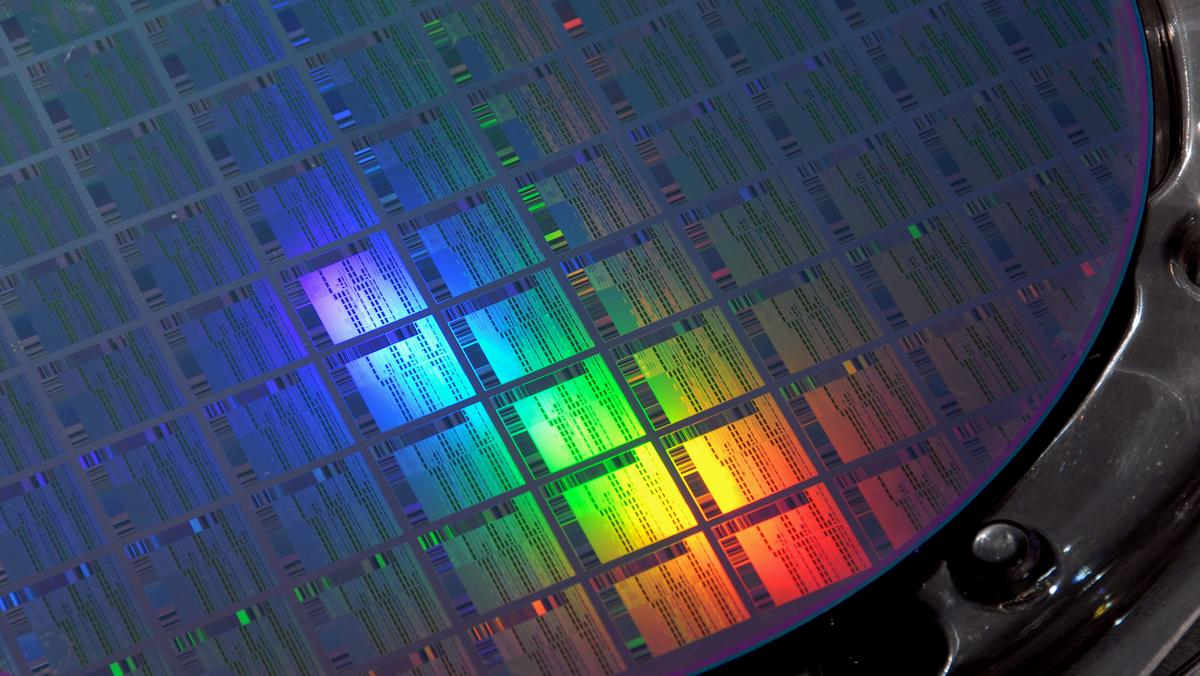
\includegraphics[scale=0.25]{Figures/oblea}}
\only<5>{\includegraphics[scale=0.5]{Figures/glóbulo-rojo}}
\only<6>{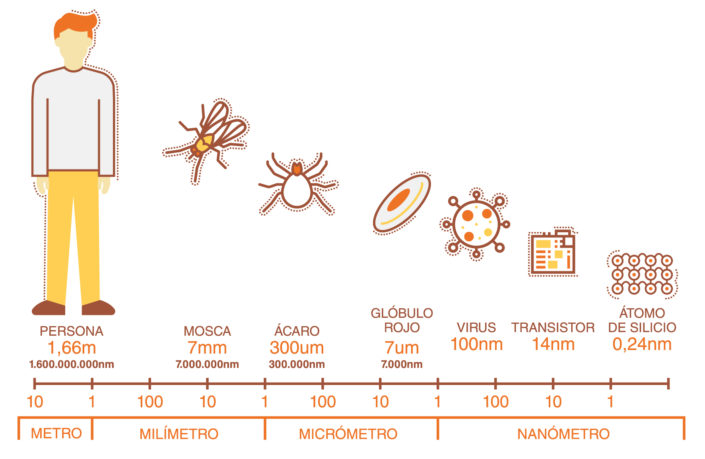
\includegraphics[scale=0.4]{Figures/tamanno}}
\only<7>{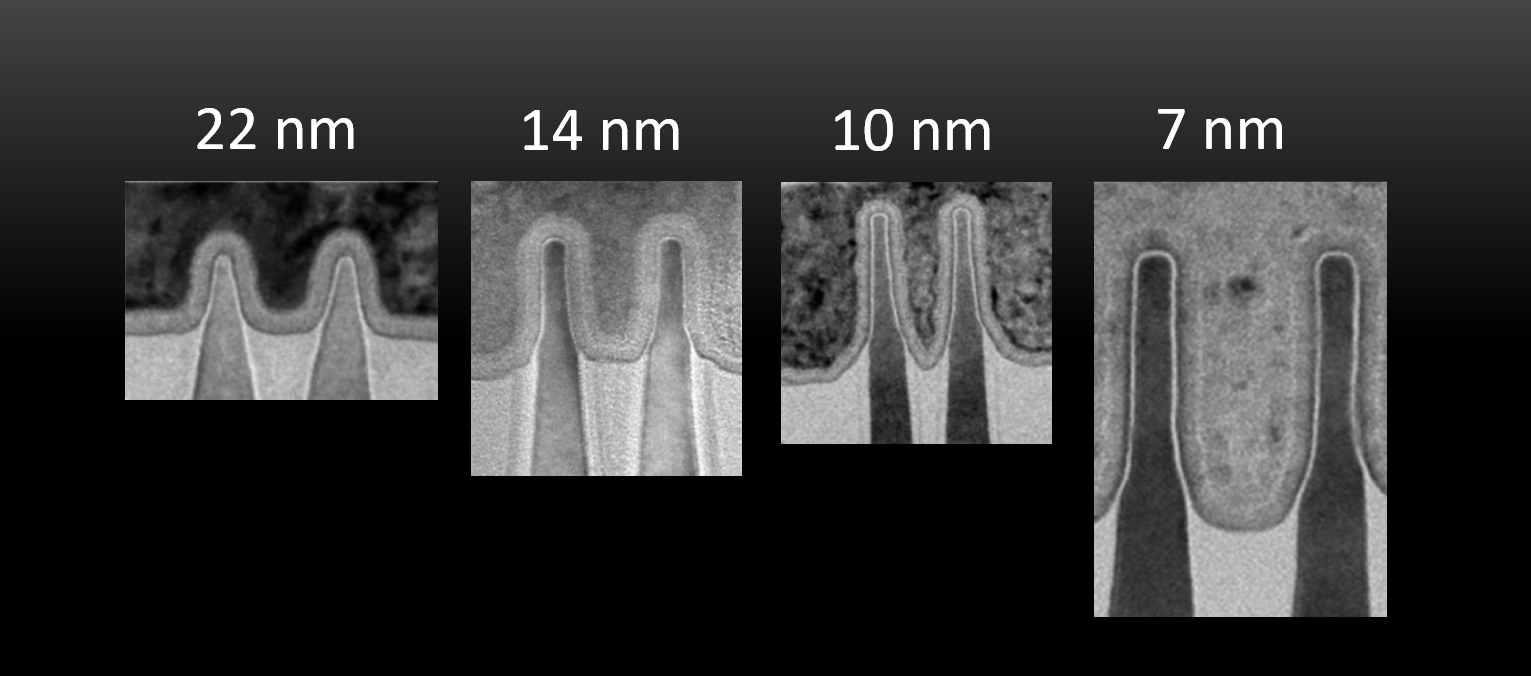
\includegraphics[scale=0.4]{Figures/Transistor}}\only<8>{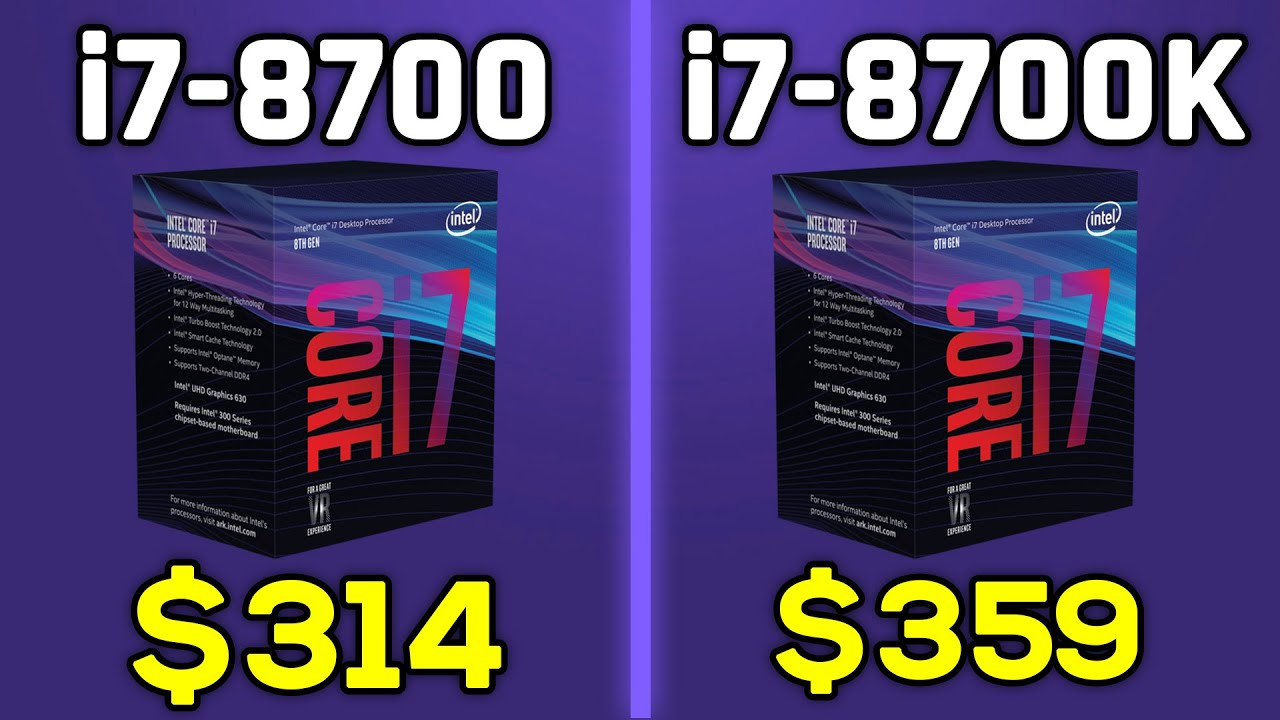
\includegraphics[scale=0.2]{Figures/8700}}
\only<9>{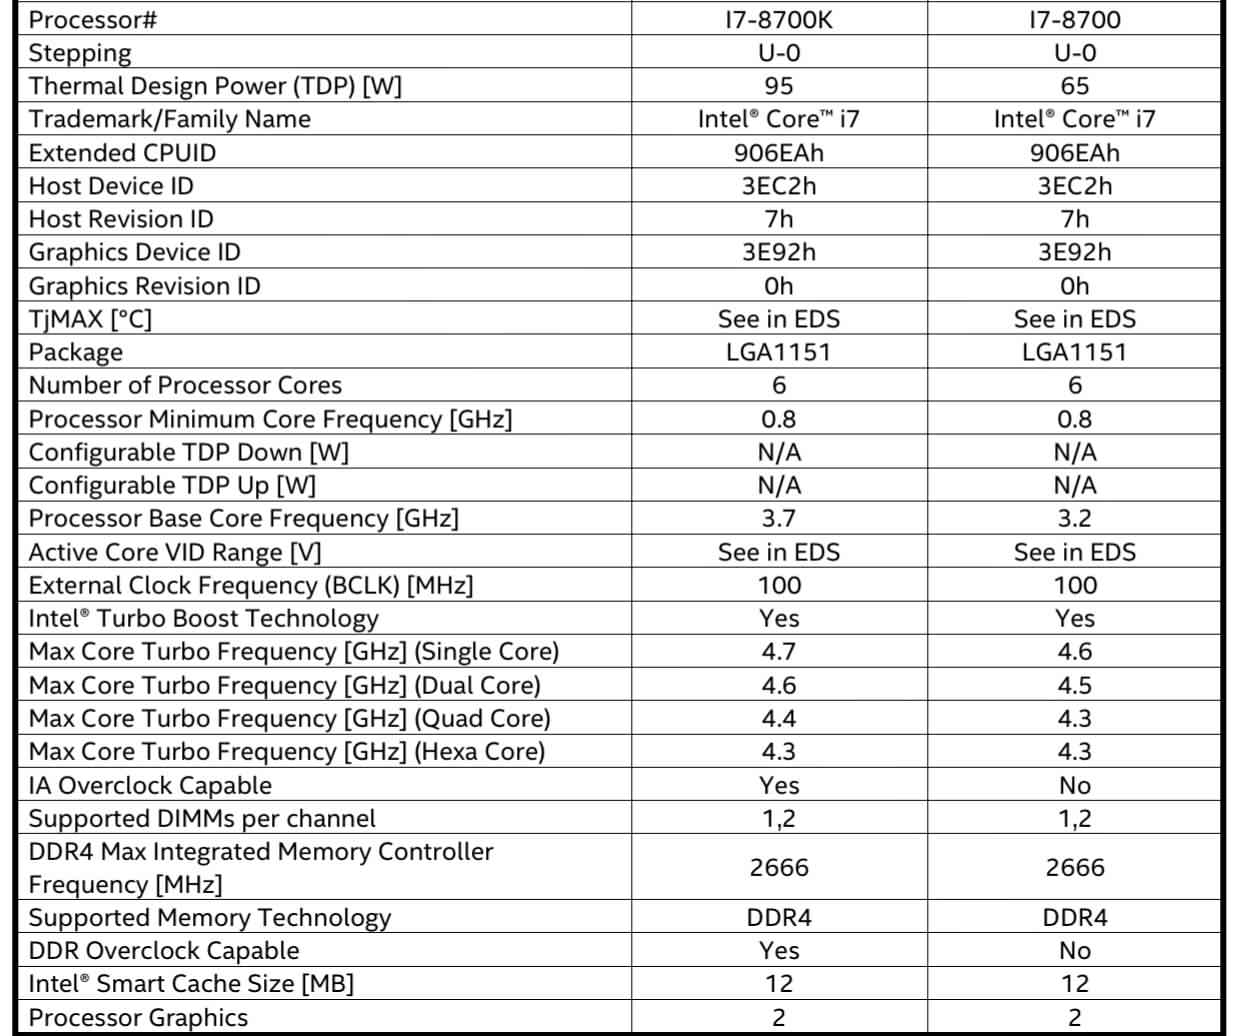
\includegraphics[scale=0.2]{Figures/8700-k}}
\end{center}
\end{frame}


\subsection{Transistor}

\begin{frame}
\begin{center}
\Huge{\textcolor{blue}{Transistor}}
\end{center}
\end{frame}

\begin{frame}{Transistor}
\begin{center}
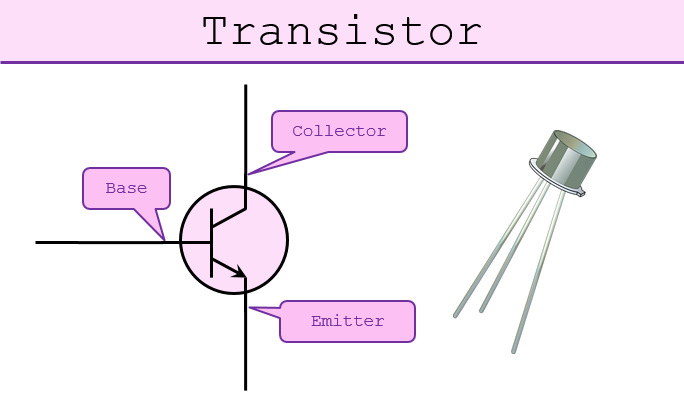
\includegraphics[scale=0.4]{Figures/4transistor}
\end{center}
\end{frame}

\begin{frame}{Tipos de transistores}
\begin{center}
\only<2>{\Large{Transistor de contacto puntual} \\ 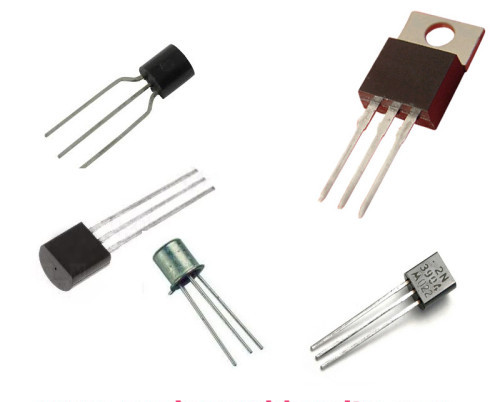
\includegraphics[scale=1.0]{Figures/TransistorPuntual} }
\only<3>{\Large{Transistor de unión bipolar} \\ 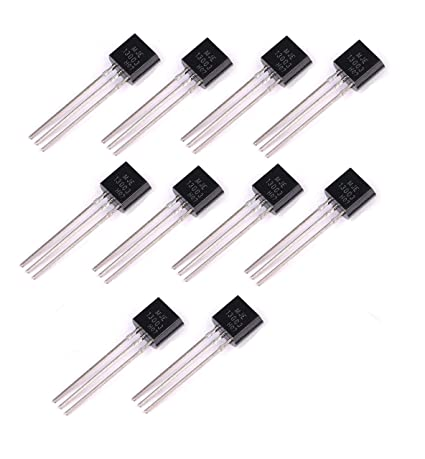
\includegraphics[scale=0.35]{Figures/bipolar} }
\only<4>{\Large{Transistor de efecto de campo} \\ 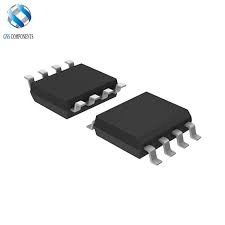
\includegraphics[scale=0.8]{Figures/campo} }
\only<5>{\Large{Fototransistores} \\ \includegraphics[scale=0.7]{Figures/fototransistor} }
\end{center}
\end{frame}

\begin{frame}{Transistor}
\begin{center}
\only<1>{\includegraphics[scale=0.3]{Figures/transistorMeme}}
\only<2>{\includegraphics[scale=0.4]{Figures/Thor}}
\end{center}
\end{frame}

\subsection{Compuertas lógicas}

\begin{frame}
\begin{center}
\Huge{\textcolor{blue}{Compuertas lógicas}}
\end{center}
\end{frame}

\begin{frame}{Compuertas lógicas}
\begin{center}
\only<2>{\Large{\textcolor{red}{AND \\}}}
\only<3>{\includegraphics[scale=0.43]{Figures/4AND-Gate}}
\only<4>{\Large{\textcolor{red}{OR \\}}}
\only<5>{\includegraphics[scale=0.43]{Figures/4OR-Gate}}
\only<6>{\Large{\textcolor{red}{NOT \\}}}
\only<7>{\includegraphics[scale=0.43]{Figures/4NOT-Gate}}
\end{center}
\end{frame}

\begin{frame}{Compuertas lógicas}
\begin{center}
\includegraphics[scale=0.7]{Figures/4puertas} \\ \pause
\tiny{\url{https://www.inventable.eu/simulador-compuertas-logicas/}}
\end{center}
\end{frame}

\begin{frame}
\begin{center}
\Large{\textcolor{blue}{Suma (Half Adder)}} \\ \vspace{1cm}
\includegraphics[scale=0.2]{Figures/4Suma} \\ \pause
\tiny{\url{http://163.10.22.82/OAS/compuertas_logicas/Simulacion/editor_simple.html}}
\end{center}
\end{frame}

\subsection{Unidades de procesamiento}

\begin{frame}
\begin{center}
\Huge{\textcolor{blue}{Unidades de procesamiento}}
\end{center}
\end{frame}

\begin{frame}{Unidades de procesamiento}
\begin{center}
\Large{\textcolor{blue}{ALU: Unidad Aritmético-Lógica }} \pause
\includegraphics[scale=0.3]{Figures/4ALU}
\end{center}
\end{frame}

\begin{frame}{Unidades de procesamiento}
\begin{center}
\Large{\textcolor{blue}{FPU: Unidad de coma flotante}} \pause
\includegraphics[scale=0.4]{Figures/4fpu}
\end{center}
\end{frame}

{\1
\begin{frame}[plain,noframenumbering]
  \finalpage{\includegraphics[scale=0.3]{Figures/Feynman}}
\end{frame}}

\end{document}